\section{Описание предметной области}

Для анализа взаимодействия CCID-токенов необходимо разработать ИС, которая позволит этот анализ провести.
Следует построить логическую модель предметной области, которая бы иллюстрировала все сущности, а также взаимоотношения между ними.

\subsection{APDU}

Коммуникация между терминалом и смарт-картой (токеном) происходит в формате APDU команд, которые описаны в ГОСТ Р ИСО/МЭК 7816
(аналоге зарубежного ISC/IEC 7816) \cite{habr-apdu}. Прикладной протокол, описанный в этом стандарте, оперирует блоками
данных которые состоят из двух подряд идущих сообщений: APDU команды (C-APDU) и APDU ответа (R-APDU) \cite{gost-7816}.
Структура любой APDU команды описана в таблице 2.1.

\begin{table}[ht]
  \begin{center}
    \resizebox{\textwidth}{!}{
      \begin{tabular}{ |l|c|l| }
        \hline
        Поле & Число байтов & Описание \\ \hline
        CLA & 1 & Байт класса CLA \\ \hline
        INS & 1 & Командный байт INS \\ \hline
        P1-P2 & 2 & Байты параметры P1-P2 \\ \hline
        $L_c$ & 0, 1 или 3 & Длина передаваемых данных \\ \hline
        Command Data & $N_c$ & Набор байтов представляющий собой передаваемые данные \\ \hline
        $L_e$ & 0, 1, 2 или 3 & Максимальное количество данных, ожидаемых в поле данных ответа \\ \hline
      \end{tabular}
    }
  \caption{Структура APDU команды}
  \end{center}
\end{table}

APDU команды начинается с байта CLA, который задает класс команды, отвечающий за параметры коммуникации. Если старший бит установлен в 1,
то это проприетарная команда, не описанная в стандарте ГОСТ Р ИСО/МЭК 7816. Следующий байт INS (командный байт) опеределяет функцию.
Полный список стандартных значений функций подробно описаны в разделе 5.1.2 вышеуказанного ГОСТ. Байты P1 и P2 задают параметры команды, и
их семантика зависит от первых двух байтов. Первые 4 байта образуют заголовок APDU команды и являются обязательными.

Формат команды ответа должен состоять как минимум из 2 байт, в которых содержится статус выполнения команды. Допустимые значения для статусов
ответа также определены в ГОСТ Р ИСО/МЭК 7816. Помимо двух зарезервированных байтов под статус ответа, R-APDU также может содержать полезную
нагрузку - данные, которые вернулись в ответ на вызов APDU команды.

\subsection{PKCS}
PKCS\#11 - один из наиболее широко применяемых в мире стандартов криптографии, описывающий платформонезависимый
интерфейс прикладного программирования (API) для криптографических токенов, которые хранят и обрабатывают аутентификацирующую
информацию пользователя, включая персональные данные, криптографические ключи, сертификаты, цифровые подписи и биометрические данные \cite{pkcs}.
API оперирует с наиболее часто используемыми в криптографии объектами: RSA ключи, сертификаты X.509 и другие, - а также описывает функции,
необходимые для работы с этими объектами.

Некоторые вендоры токенов позволяют разработчикам взаимодействовать со своими устройствами, предоставляя собственные библиотеки, использующие
стандарт PKCS\#11 \cite{esmart-pkcs,rutoken-pkcs,alladin-pkcs}. Схема взаимодействия показана на рис. 1: сначала 
вызывается функция из библиотеки, которую предоставил вендор устройства, затем делается запрос к PKCS\#11 API,
и в итоге пакеты в формате APDU команд передаются на смарт-карту, либо токен.

\begin{figure}[H]
  
\includegraphics[scale=0.5]{images/apdu-pkcs.png}
  \caption{Взаимодействие со смарт-картой}
  \label{apdu}
\end{figure}

Стандарт обладает рядом преимуществ \cite{pkcs-cons-pros}:
\begin{itemize}
  \item кросплатформенность
  \item высокий уровень абстракции
  \item простой интерфейс для языка C
\end{itemize}

Тем не менее, стандрат также имеет и недостатки, которые стоит учесть при разработке стенда. Значимым недостатком является отсутствие
полноценной поддержки стандарта операционными системами семейства Windows и, как следствие, прикладным программным обеспечением под Windows.

Для работы с PKCS\#11 API приложение инициирует сеанс с токеном, предоставляя PIN-код. Стоит учитывать, что если на хост-машине запущен
вредоносный код, то PIN-код пользователя может быть легко перехвачен, например с помощью кейлогера или поддельного CCID-драйвера устройства,
позволяя злоумышленнику инициировать свои собственные сеансы с устройством.
Тем не менее, стандарт был разработан для защиты конфиденциальных данных даже в тех случаях, если устройство
подключено к скомпрометированному считывателю. Для этих целей вводятся дополнительные меры безопасности в виде аттрибутов, которыми
помечаются ключи, хранящиеся на устройстве, и которые не позволяют читать их содержимое открытым текстом \cite{pkcs-standard}.
После инициирования сессии приложение может получить доступ к объектам, хранящимся на токене, например, ключам и сертификатам.

Несмотря на меры безопасности, предполагающие работу с компрометированным хостом, существует описание атак,
которые могут приводить к краже конфиденциальных данных, поэтому анализ защищенности
токенов является актуальной задачей и по сей день \cite{attack-fix-pkcs}.

\subsection{Анализаторы траффика CCID-токенов}

Поскольку основной задачей предпроектного исследования является анализ взаимодействия с аппаратными CCID-токенами, то следует
рассмотреть инструментарий, с помощью которого анализ будет проведен. А именно, существующие анализаторы USB траффика. На сегодняшний день
на рынке распространены анализаторы двух видов: программные и аппаратные.

Программные анализаторы заменяют собой программный стек протокола USB на хост-машине, чтобы контролировать и отслеживать данные,
идущие с периферийного устройства. Как следствие, такие анализаторы полностью зависят от аппаратного обеспечения хостовой ЭВМ,
а именно хост-контроллера USB. Хост-контроллер отвечает за коммуникацию с периферийными устройствами, а также за управление действиями,
такими как повторная передача данных при ошибках. Контроль выполнения таких действий осуществляется внутри хост-контроллера USB, и поэтому
они не входят в компетенцию каких-либо анализаторов трафика.\cite{hardware-analyzer}

Преимущества аппаратного анализатора траффика заключаются в:
\begin{itemize}
  \item Независимости от хост-машины, на которой производится анализ, поскольку мониторинг не нуждается во взаимодействии с шиной USB
  \item Возможности отслеживать низкоуровненые состояния шины USB и ошибки
  \item Возможности добавления точек останова при анализе трафика
  \item Высокой временной точности мониторинга событий
\end{itemize}

Однако, большинство решений на рынке являются довольно дорогостоящими. К тому же, ни один из производителей не заявляет поддержку
стандарта CCID, лишь HID (Human Interface Device) и Mass Storage \cite{beagle,ellisys,lecroy}.

Программные анализаторы USB трафика в большинстве своем являются бесплатными проектами, поддерживающими как ОС семейства Windows,
так и ОС Linux. Эти программы устанавливает свой собственный драйвер между драйвером хост-контроллера USB и драйвером устройства,
а затем отслеживает все блоки запросов USB (USB Request Blocks), отображая их пользователю в легко читаемом формате \cite{windows-analyzer}.
Программные анализаторы позволяют:
\begin{itemize}
  \item контролировать траффик, проходящий через шину USB
  \item декодировать и отображать данные
  \item проводить обратную разработку USB протоколов, устройств, драйверов и приложений
\end{itemize}

Наиболее подходящие программные аналазиторами для решения поставленной задачи перечислены в таблице 2.2.

\begin{table}[ht]
  \begin{center}
    \resizebox{\textwidth}{!}{
      \begin{tabular}{ |l|c|c|c| }
        \hline
        Название & Описание & Поддержка windows & Поддежка Linux \\ \hline
        Wireshark & Известный всем & + & + \\ \hline
        Free USB Analyzer & asd & + & - \\ \hline
        APDUPlay & some description & + & + \\ \hline
        pcsc-tools & debian tools & - & + \\ \hline
      \end{tabular}
    }
  \caption{Программные анализаторы}
  \end{center}
\end{table}

\subsection{Компоненты системы}

Для разработки стенда необходимым аппаратным обеспечением являются ЭВМ, на которой будет проводиться анализ, а также CCID-токен.
Как уже отмечалось выше, ОС семейства Windows не имеют полноценной поддержки протола PKCS\#11. К тому же, в ОС семейства Linux, а именно Debian,
имеется встроенный набор утилит для взаимодействия с аппаратными CCID-токенами, поэтому хостовой ОС на ЭВМ будет Linux Debian 10.5,
имеющая последнюю мажорную версию ядра Linux и поддерживаемая разработчиками.

Наглядно-графическая модель системы представлена на рис. 2.

\begin{figure}[H]
  \hfill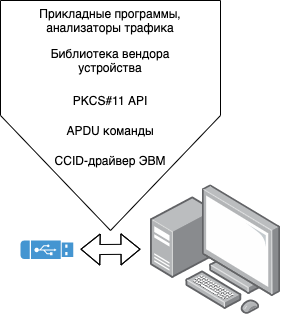
\includegraphics[scale=0.8]{images/general.png}\hspace*{\fill}
  \caption{Схематическое представление предметной области}
\end{figure}

\subsection{Анализ уязвимостей при взаимодействии с CCID-токенами}

При работе с токенами, либо смарт-картами происходит обмен конфиденциальной информацией между токеном и сторонними системами. Такой обмен
подвержден атакам типа "человек посередине", что делает токены уязвимыми. Анализ трафика CCID-токенов привлек много внимания и
впоследствии было предложено множество инструментов. Например, некоторые из работ показали, что знание семантики взаимодействия с токеном
может позволить злоумышленнику \cite{smart-logic, smart-detective}:
\begin{itemize}
  \item получить PIN-код или другие аутентифицирующие данные в открытом виде
  \item получить доступ к конфиденциальным ключам
  \item выполнять несанкционированные операции
  \item клонировать токен или карту
\end{itemize}

\clearpage